\documentclass[handout,nooutcomes]{ximera}
%% handout
%% space
%% newpage
%% numbers
%% nooutcomes


\newcommand{\RR}{\mathbb R}
\renewcommand{\d}{\,d}
\newcommand{\dd}[2][]{\frac{d #1}{d #2}}
\renewcommand{\l}{\ell}
\newcommand{\ddx}{\frac{d}{dx}}
\newcommand{\dfn}{\textbf}
\newcommand{\eval}[1]{\bigg[ #1 \bigg]}

\usepackage{multicol}

\renewenvironment{freeResponse}{
\ifhandout\setbox0\vbox\bgroup\else
\begin{trivlist}\item[\hskip \labelsep\bfseries Solution:\hspace{2ex}]
\fi}
{\ifhandout\egroup\else
\end{trivlist}
\fi} %% we can turn off input when making a master document

\title{Recitation \#3 - 2.2:  Definition of Limits}  

\begin{document}
\begin{abstract}		\end{abstract}
\maketitle

\section*{Warm up:} 

	\begin{enumerate}[label=(\alph*)]
	
	\item  True or False: To find $\lim_{x \to 2} f(x)$, it's enough to know $f(2.1)$, $f(2.01)$, $f(2.001)$, etc.
	\begin{freeResponse}
	 False.  These values will only help us make a guess at $\lim_{x \to 2^+} f(x)$, the right hand limit of $f(x)$.  To determine $\lim_{x \to 2} f(x)$, we also need to know $\lim_{x \to 2^-} f(x)$ which we cannot determine from the above values.  For example, consider the function
	 	\begin{image}
	 	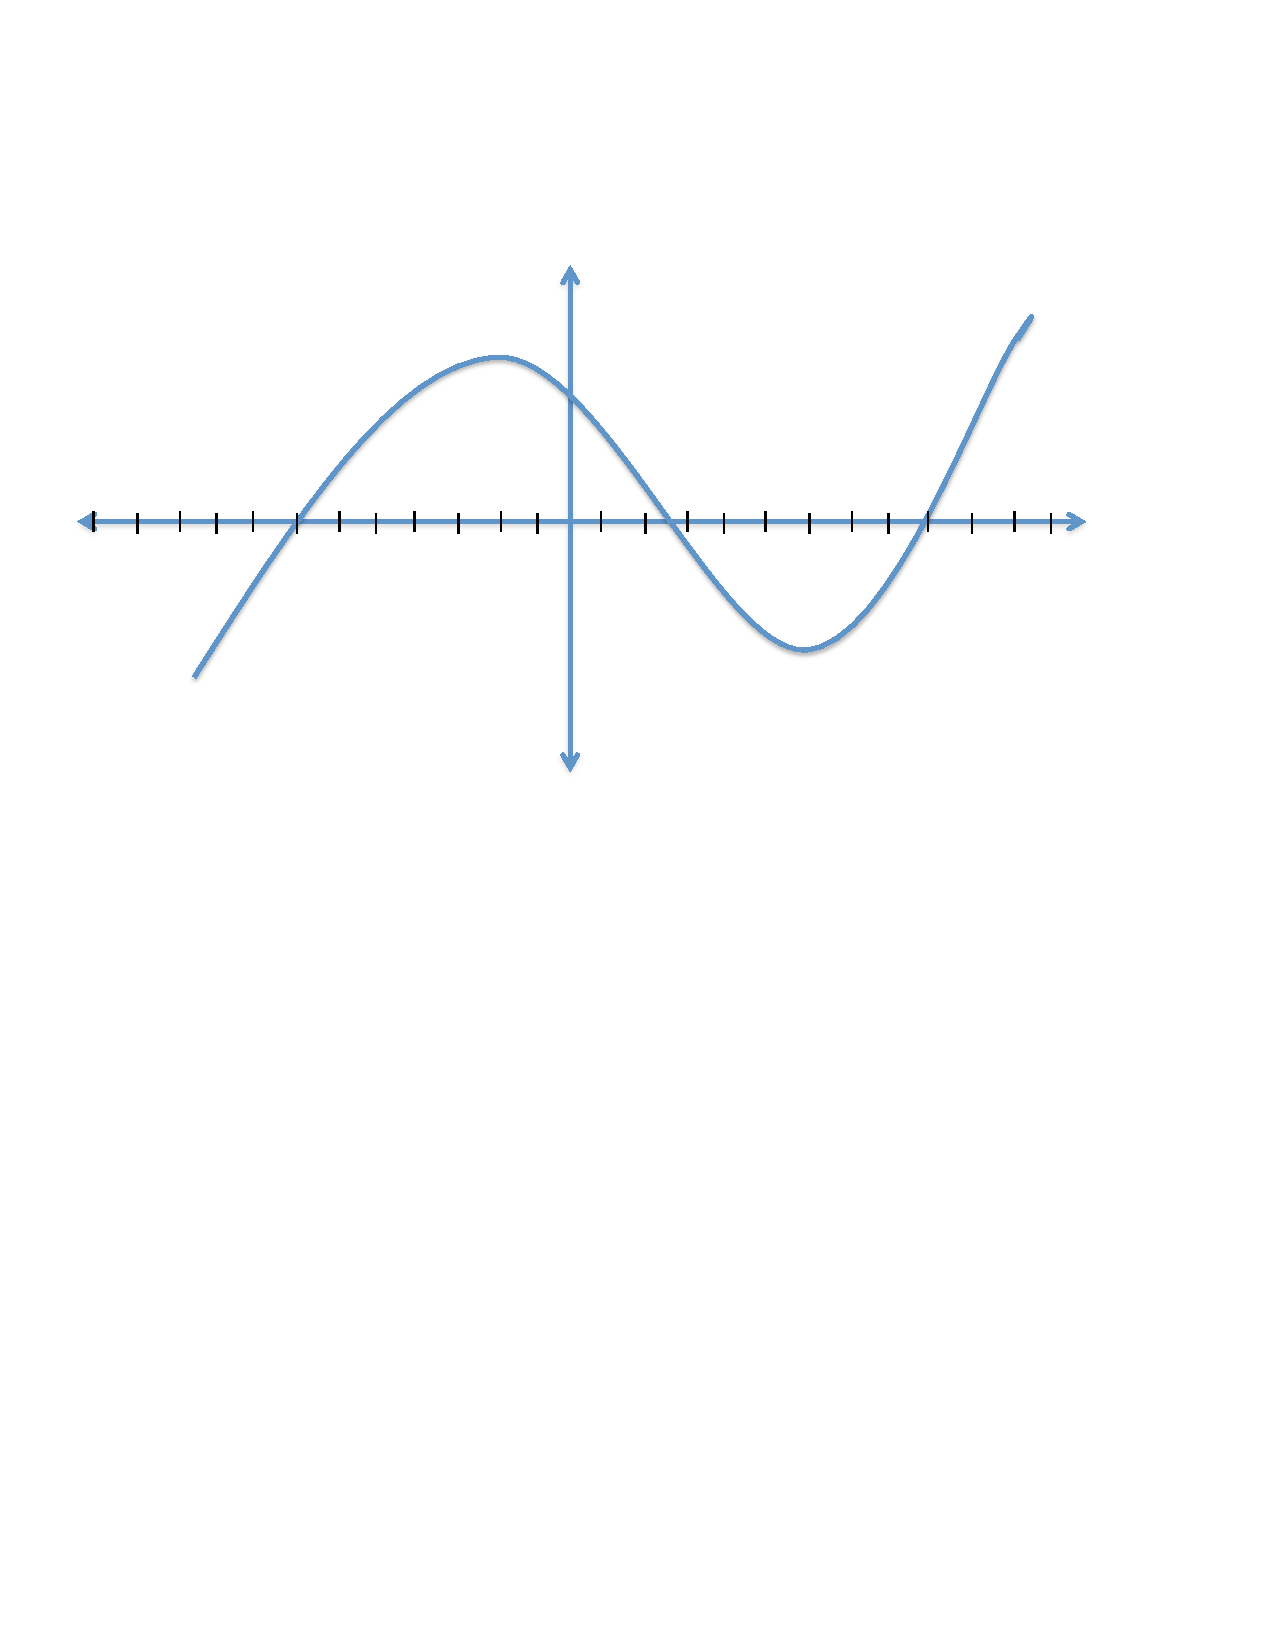
\includegraphics[trim= 70 570 300 165]{Figure2.pdf}
	 	\end{image}
	 	
	Looking at the graph of this function below, we can see that $\lim_{x \to 2^+} f(x) = 1$ and $\lim_{x \to 2^-} f(x) = -1$.  Thus, since $\lim_{x \to 2^+} f(x) \neq \lim_{x \to 2^-} f(x)$, $\lim_{x \to 2} f(x)$ does not exist.
	
		\begin{image}
		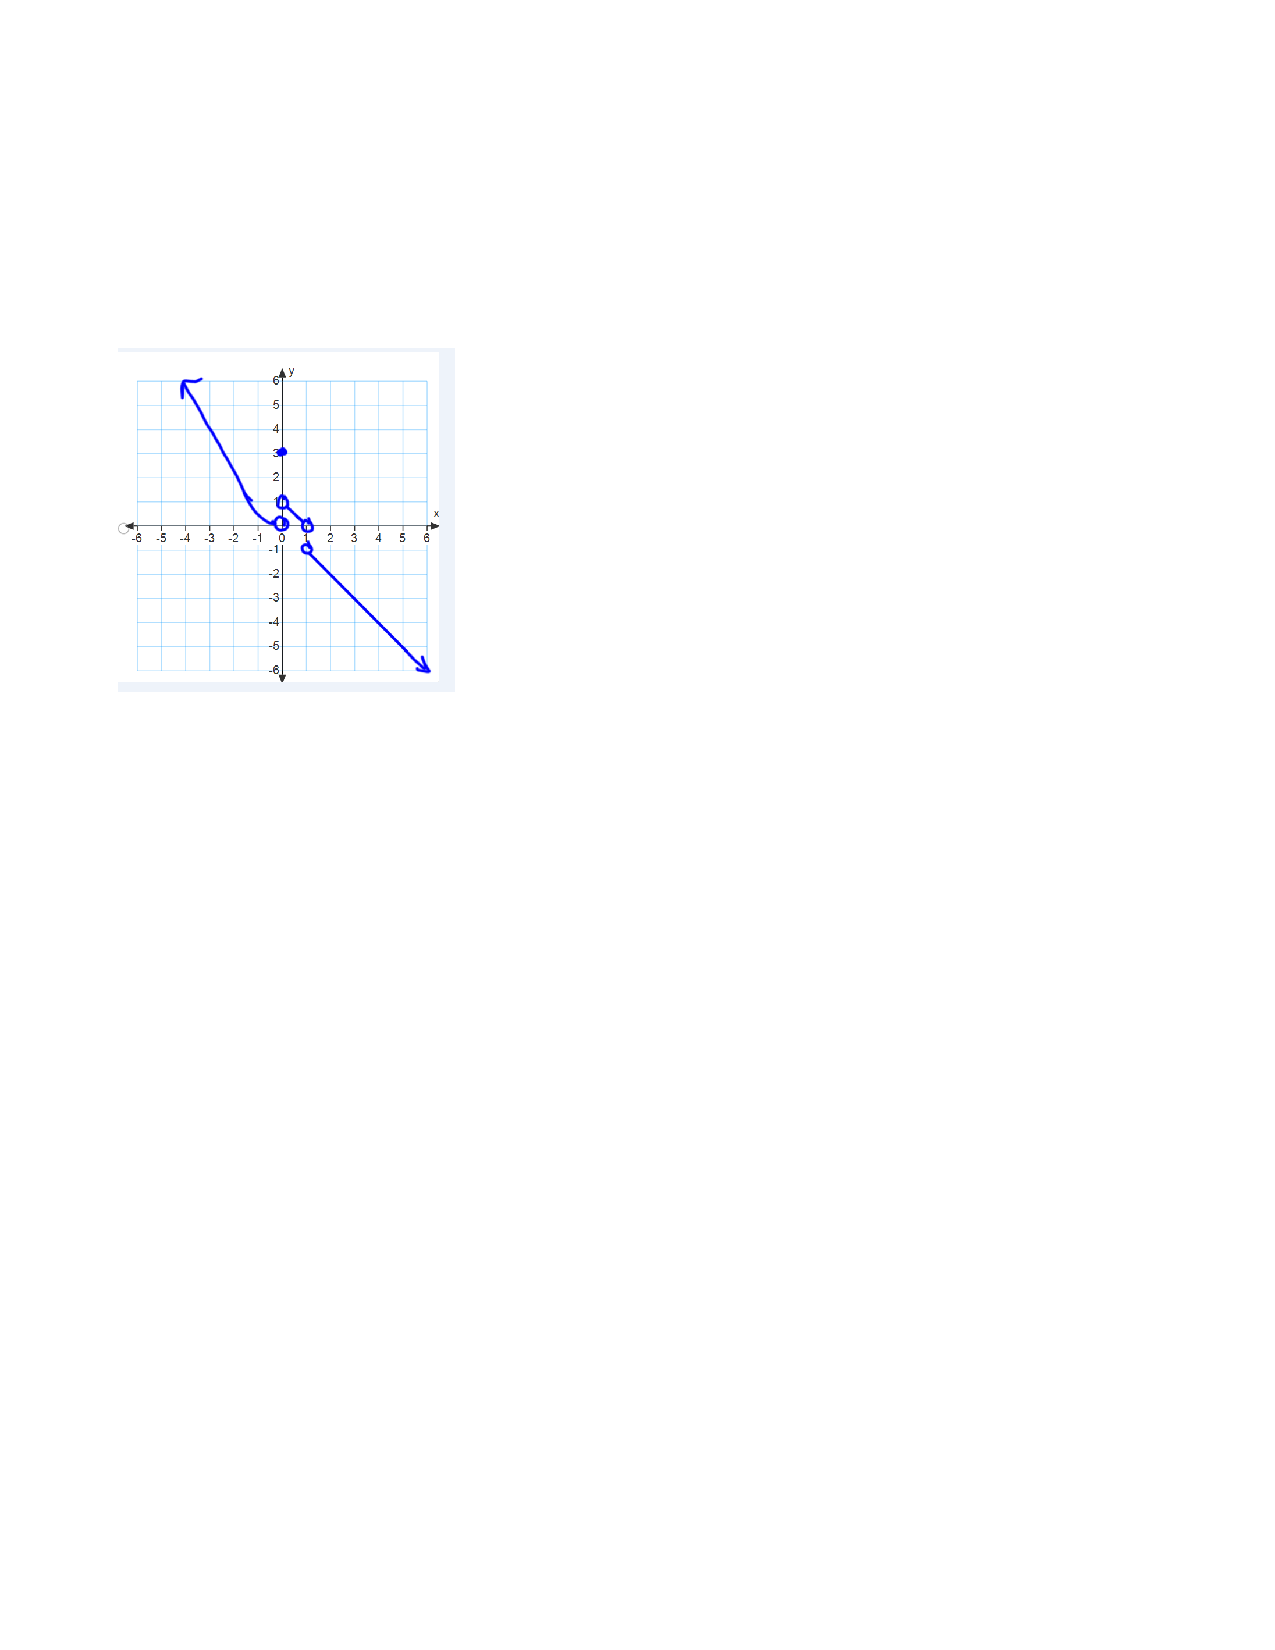
\includegraphics[trim= 70 470 250 160]{Figure3.pdf}
		\end{image}
	\end{freeResponse}
	
	
	
	\item  True or False: If we know $f(2)$, then we know $\lim_{x \to 2} f(x)$.
		\begin{freeResponse}
		False.  In the above example, we have that $f(2) = 0$, however $\lim_{x \to 2} f(x)$ does not exist.
		\end{freeResponse}
	\end{enumerate}



\section*{Group work:}

%Problem 1	
\begin{problem}
Given the graph of the function, estimate $\lim_{x \to 1} \frac{x^2 - 1}{x - 1} $.  Then estimate $\lim_{x \to 1} \frac{x^2 - 1}{x - 1} $ by creating a table of values.
	
	\begin{image}
	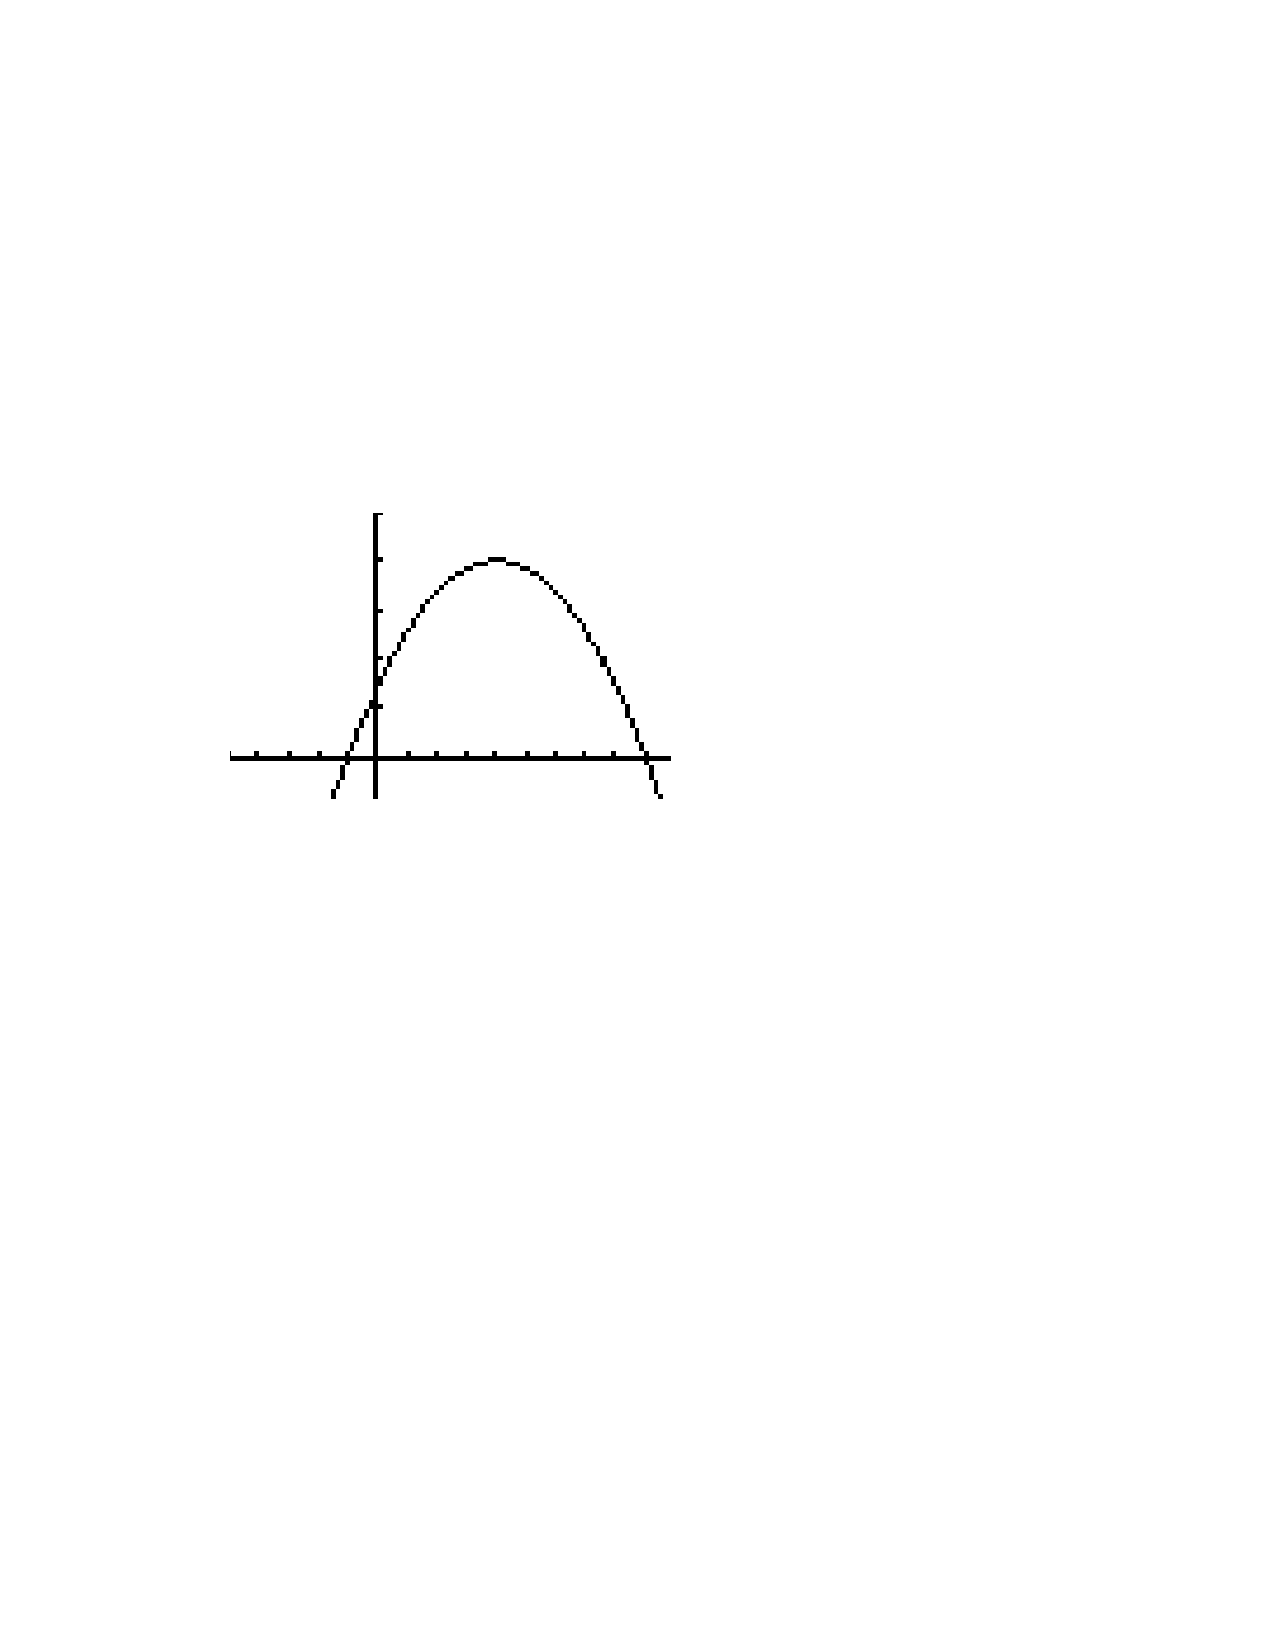
\includegraphics[trim= 50 470 300 135]{Figure1.pdf}
	\end{image}
	
	\begin{freeResponse}
	From the graph and table of values, it appears as though $\lim_{x \to 1} f(x) = 2$.
	
	\begin{tabular}{|l|l|}
	\hline
	\hspace{2mm} $x$ & \hspace{4mm} $f(x)$  \\
	\hline
	.9 & $ \frac{{{.9}^{2}}-1}{.9-1}=1.9  $  \\
	\hline
	.99 & $ \frac{{{.99}^{2}}-1}{.99-1}=1.99 $  \\
	\hline
	.999 & $ \frac{{{.999}^{2}}-1}{.999-1}=1.999 $  \\
	\hline
	1.1 & $ \frac{{{1.1}^{2}}-1}{1.1-1}=2.1 $  \\
	\hline
	1.01 & $ \frac{{{1.01}^{2}}-1}{1.01-1}=2.01 $  \\
	\hline
	1.001 & $ \frac{{{1.001}^{2}}-1}{1.001-1}=2.001 $  \\
	\hline
	\end{tabular}
	
	\end{freeResponse}
	
\end{problem}
			
			
			

%Problem 2
\begin{problem}
Sketch the graph of a function with the given properties.  You need not find a formula for the function.
	$$ f(3) = -2 , f(5) = 6 , \lim_{x \to 5^-} f(x) = -1 ,   \lim_{x \to 5^+} f(x) = 4 ,  \lim_{x \to 3} f(x) = 7 $$
	$$  \lim_{x \to -2^-} f(x) = 3 ,  \lim_{x \to -2^+} f(x) = 0 ,  \lim_{x \to 1^+} f(x) = 5  $$
	\begin{freeResponse}
	While there are many correct solutions to this problem, one example can be seen below.
	
		\begin{image}
		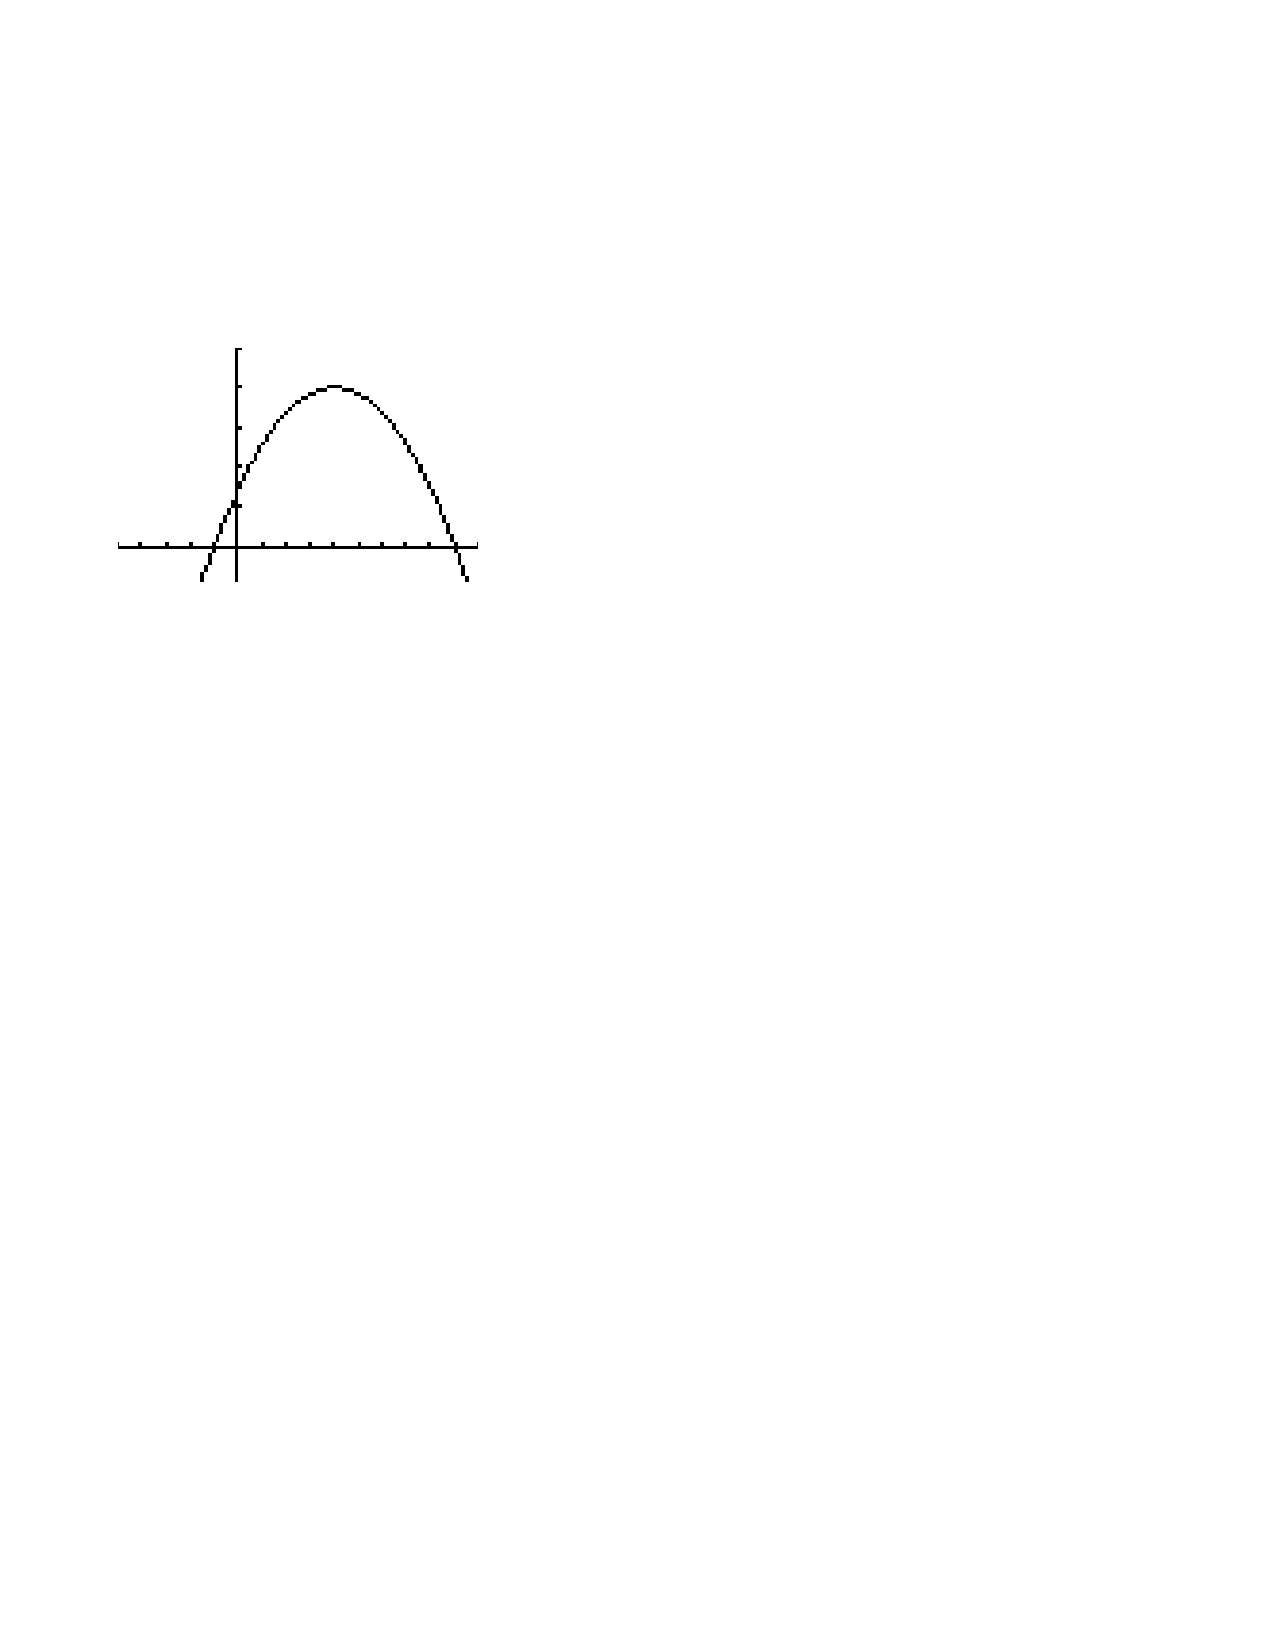
\includegraphics[trim= 70 470 250 160]{Figure4.pdf}
		\end{image}
	\end{freeResponse}
\end{problem}
	
	
	
	

%Problem 3	
\begin{problem}
True/False:  Give an explanation or counterexample.  Assume $a$ and $L$ are finite numbers.
	
			\begin{enumerate}
			
			%part a
			\item  If $ \lim_{x \to a} f(x) = L$, then $f(a) = L$.
			\begin{freeResponse}
			False.  In the graph below $ \lim_{x \to 1} f(x) = 2 $, but $f(1)$ does not exist.
			
				\begin{image}
				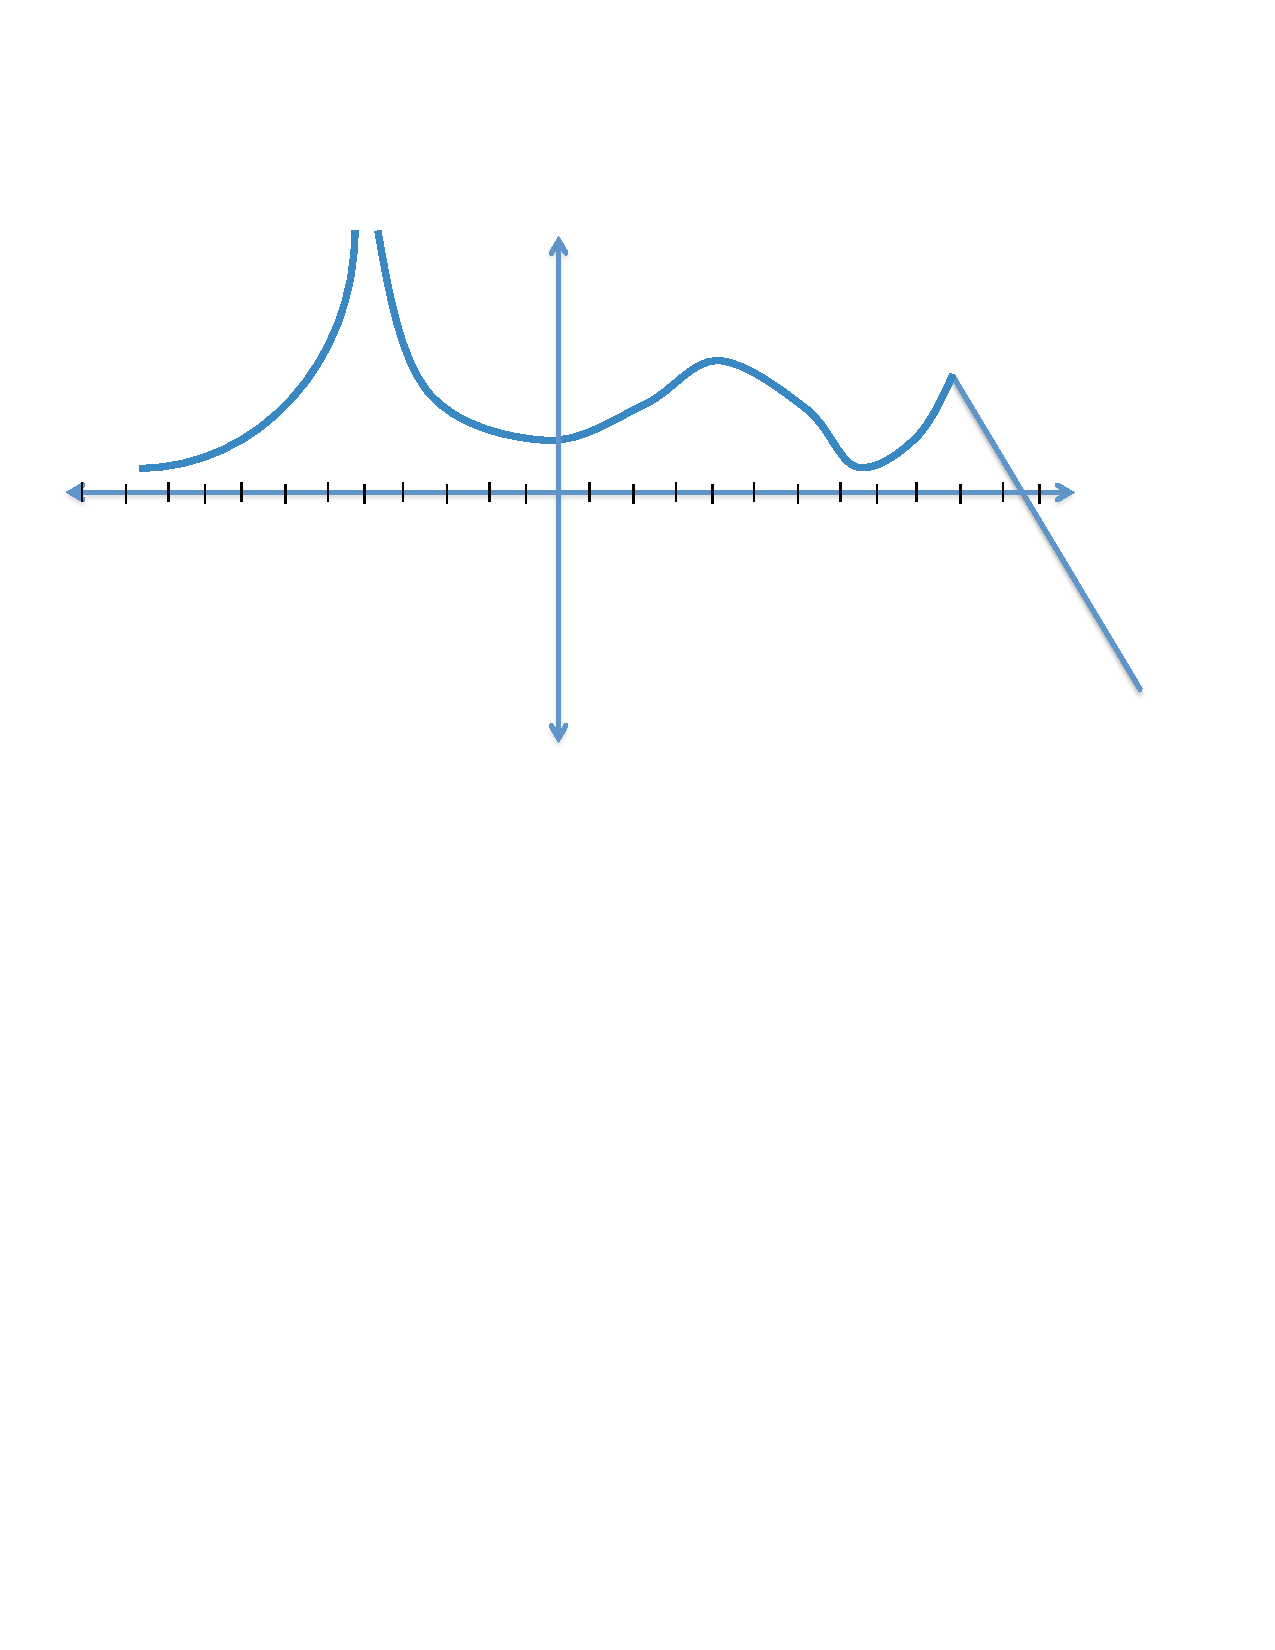
\includegraphics[trim= 70 470 250 160]{Figure5.pdf}
				\end{image}
			\end{freeResponse}
			
			
			
			%part b
			\item  If $  \lim_{x \to a^-} f(x) = L$, then $  \lim_{x \to a^+} f(x) = L $.
			\begin{freeResponse}
			False.  In the graph below $ \lim_{x \to 1^-} f(x) = 5$ but $ \lim_{x \to 1^+} f(x) = 6$.
			
				\begin{image}
				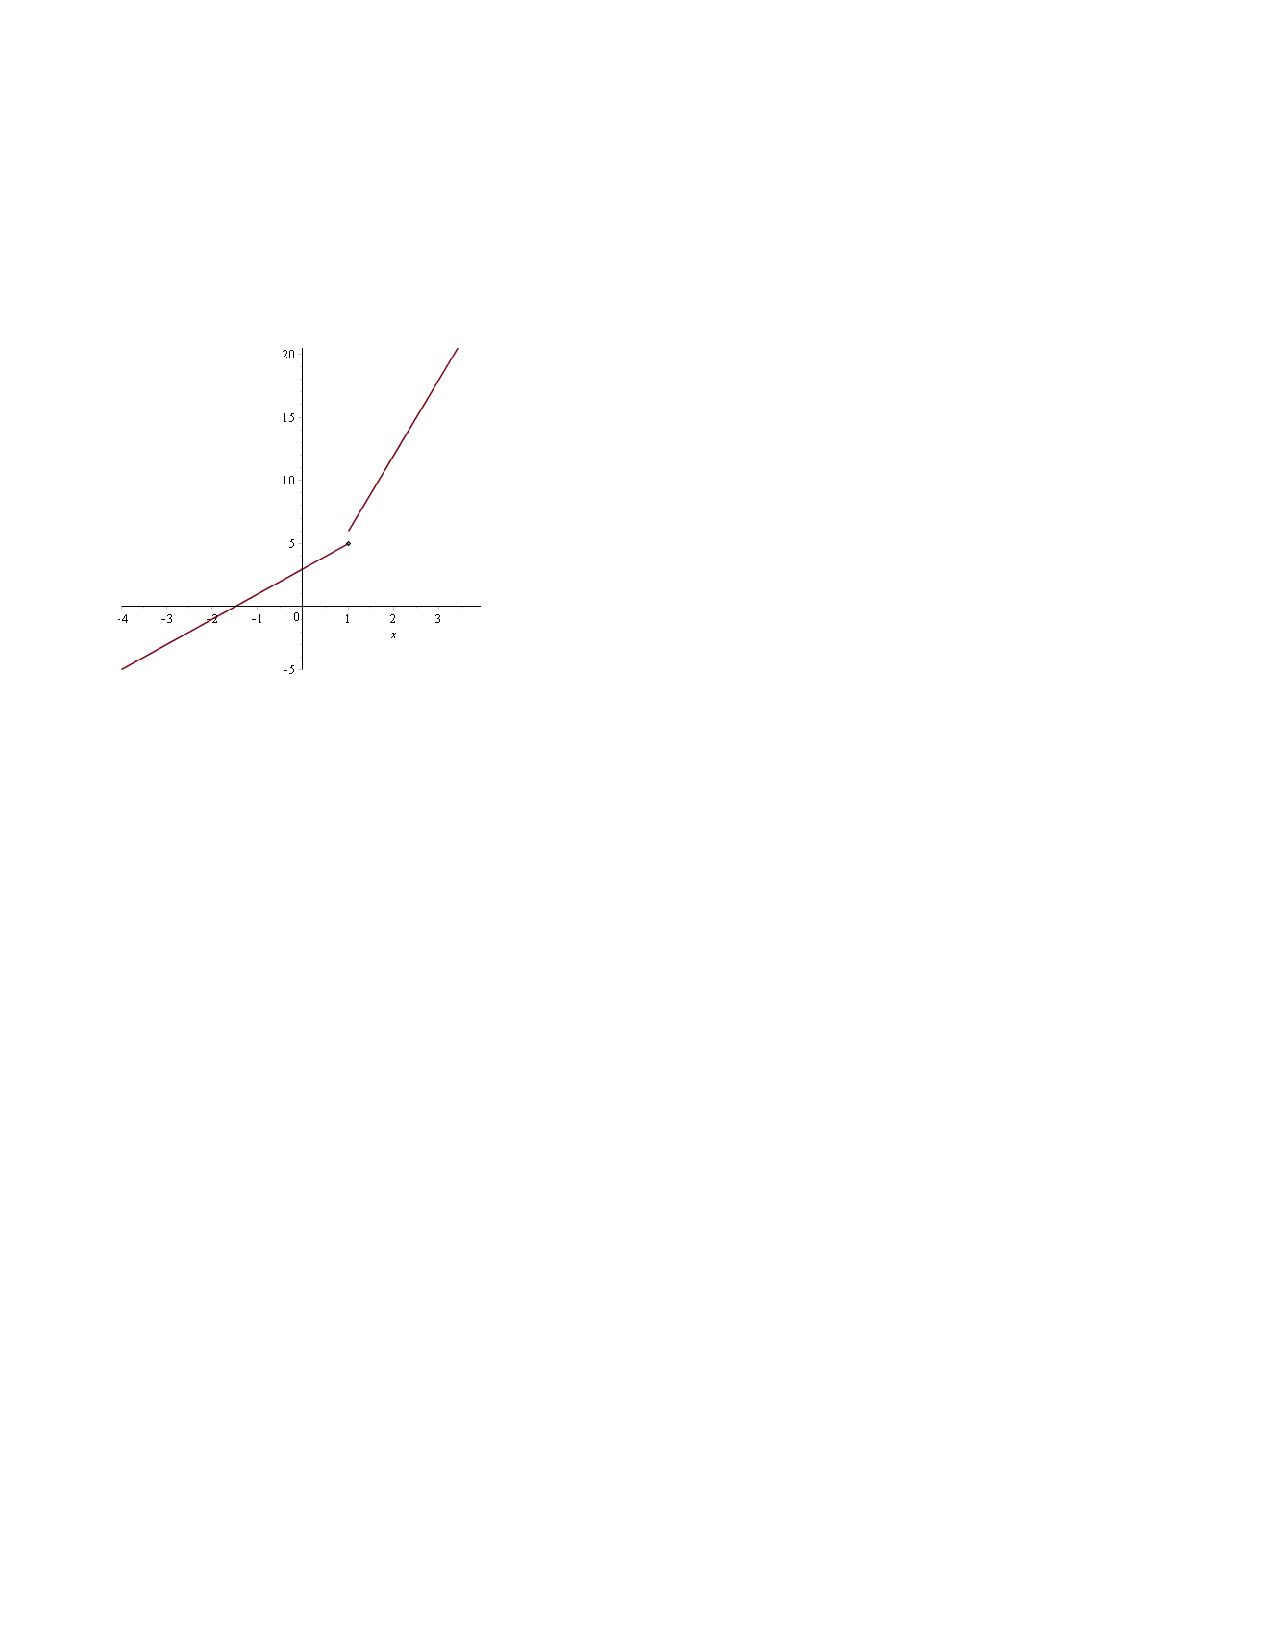
\includegraphics[trim= 70 470 250 160]{Figure6.pdf}
				\end{image}
			\end{freeResponse}
			
			
			
			%part c
			\item  If $ \lim_{x \to a} f(x) = L $ and $  \lim_{x \to a} g(x) = L $, then $f(a) = g(a)$.
			\begin{freeResponse}
			 False.  If we let 
			 
			 	\begin{image}
			 	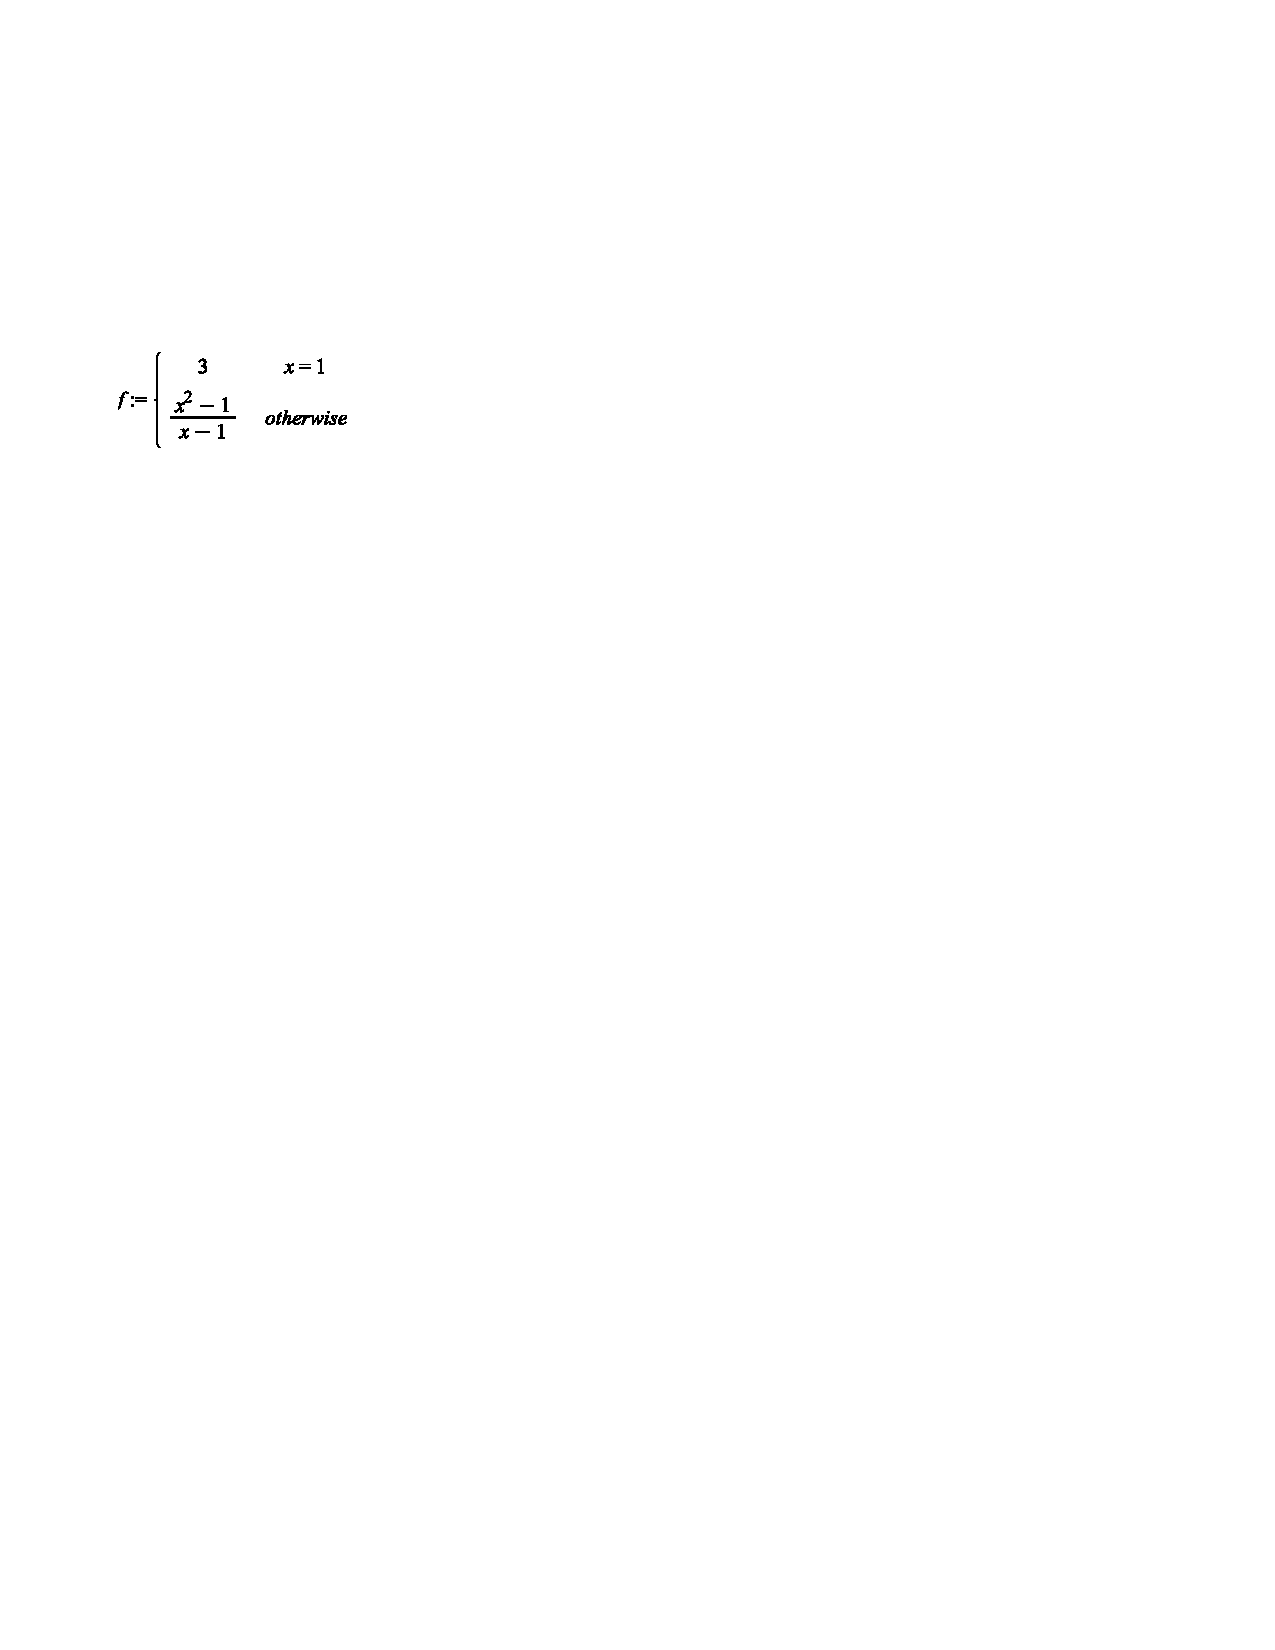
\includegraphics[trim= 70 575 300 165]{Figure7.pdf}
			 	\end{image}
			 	
			and
			
				\begin{image}
				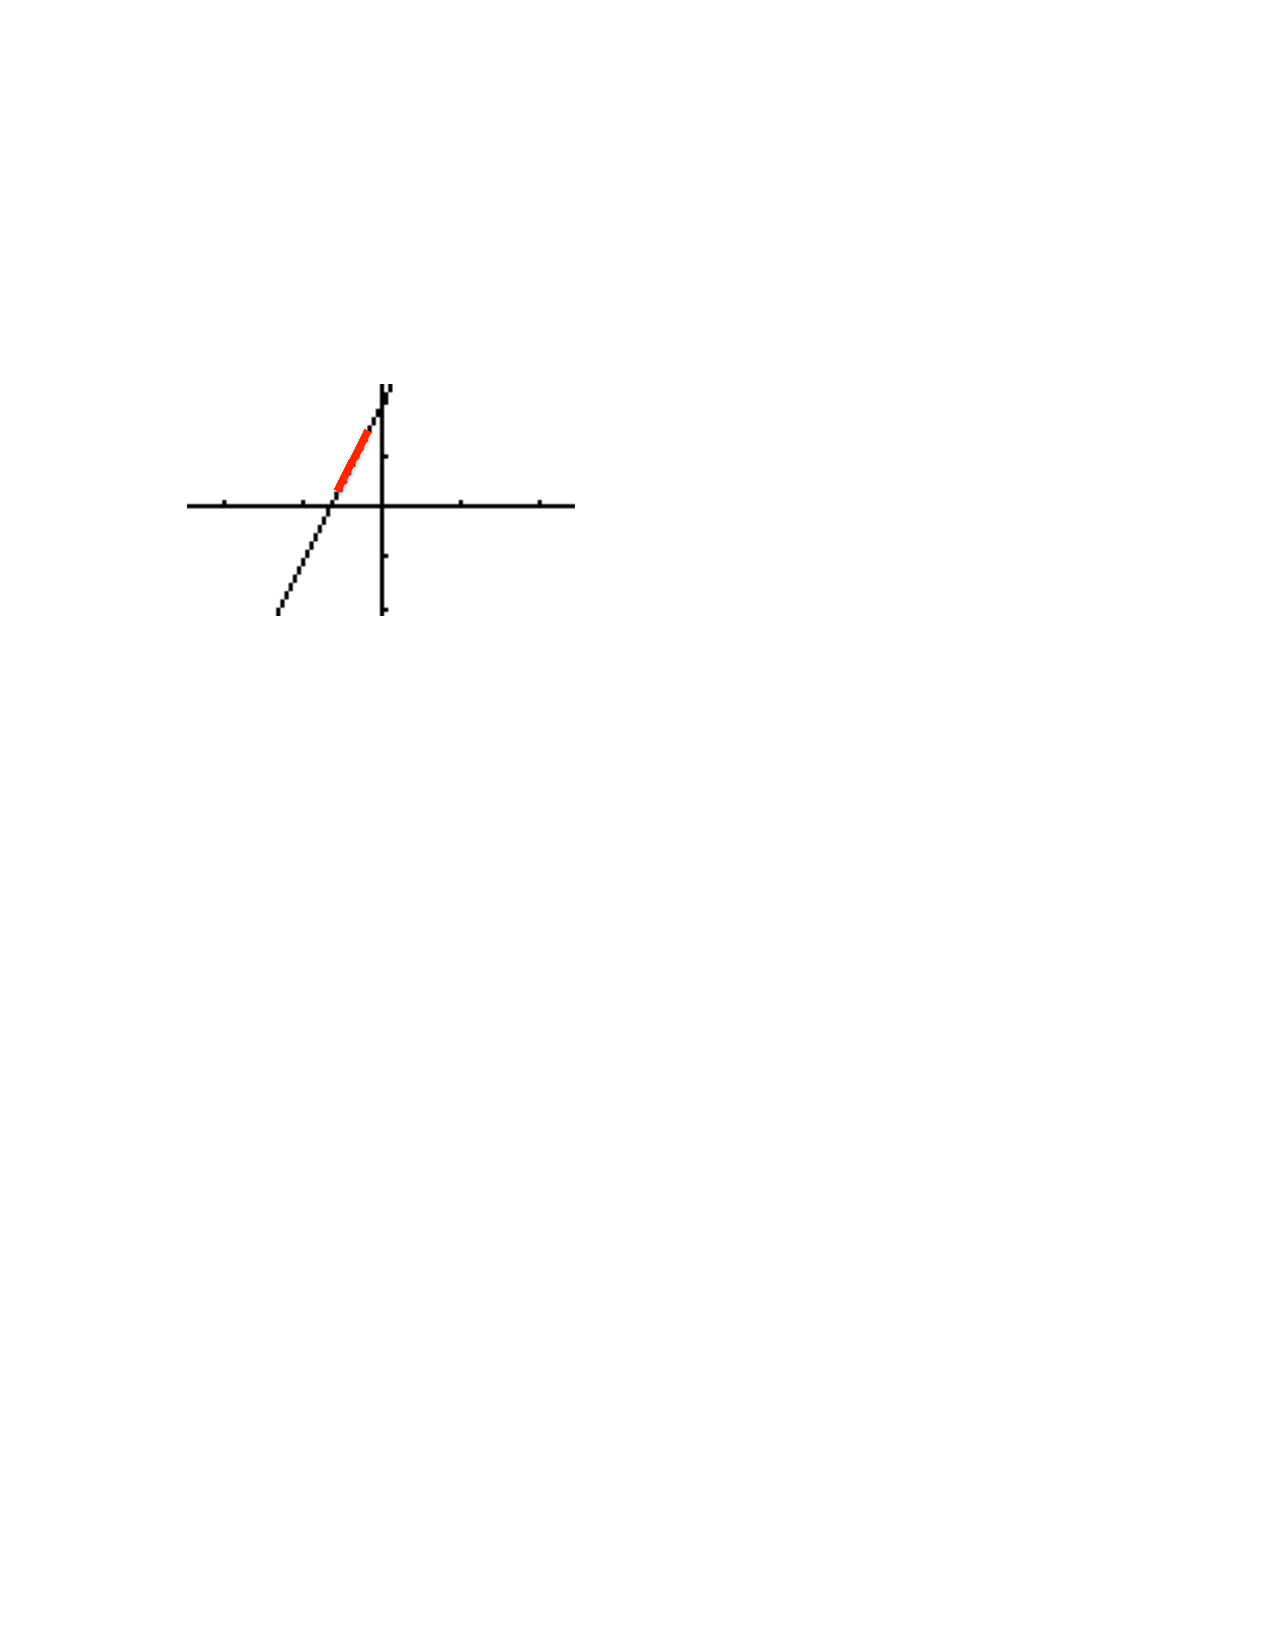
\includegraphics[trim= 70 580 300 165]{Figure8.pdf}
				\end{image}
				
			 we see that $ \lim_{x \to 1} f(x) = \lim_{x \to 1} g(x) = 2$, but $f(1) = 3$ and $g(1) = 1$.
			\end{freeResponse}
			
			
			
			%part d
			\item  $ \lim_{x \to a} \frac{f(x)}{g(x)} $ does not exist if $g(a) = 0$.
			\begin{freeResponse}
			False.  If $f(x) = x^3$ and $g(x) = x^2$, then $g(0) = 0$ but $ \lim_{x \to 0} \frac{f(x)}{g(x)} = \lim_{x \to 0} \frac{x^3}{x^2} = \lim_{x \to 0} x = 0$.  
			\end{freeResponse}
			
			
			
			\end{enumerate}
\end{problem}
	










								
				
				




























\end{document} 


















